\documentclass[tikz,border=1.35mm]{standalone}

\definecolor{fvmadaptedge}{HTML}{8A7E7E}

\definecolor{splitred}{HTML}{AF2525}
\definecolor{splitgreen}{HTML}{0E8814}

% One quadrilateral child face highlighted inside a split triangle.
% Coordinates are in millimeters; y=-1mm keeps the SVG-style origin at top left.
\begin{document}
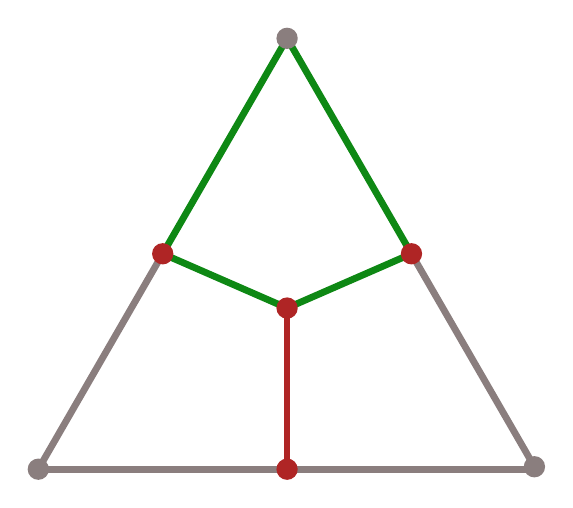
\begin{tikzpicture}[
  x=1mm,
  y=-1mm,
  line join=round,
  edge/.style={draw=fvmadaptedge,line width=0.865mm},
  splitline/.style={draw=splitred,line width=0.865mm},
  greenedge/.style={draw=splitgreen,line width=0.865mm}
]
  % Match the original artwork frame before the standalone border is applied.
  \useasboundingbox (0,0) rectangle (65.711,57.425);

  % Original triangle vertices plus split-created edge midpoints and face center.
  \coordinate (left) at (1.353,56.073);
  \coordinate (right) at (64.538,56.073);
  \coordinate (top) at (32.945,1.353);
  \coordinate (leftMid) at (17.149,28.713);
  \coordinate (rightMid) at (48.741,28.713);
  \coordinate (bottomMid) at (32.945,56.073);
  \coordinate (center) at (32.945,35.609);

  % Green edges indicate the selected quadrilateral child face.
  \draw[greenedge] (top) -- (leftMid);
  \draw[greenedge] (top) -- (rightMid);
  \draw[greenedge] (leftMid) -- (center) -- (rightMid);

  % Remaining boundary topology is drawn in #8a7e7e.
  \draw[edge] (left) -- (leftMid);
  \draw[edge] (left) -- (bottomMid) -- (right);
  \draw[edge] (rightMid) -- (right);
  \draw[splitline] (center) -- (bottomMid);

  % Original vertices are #8a7e7e.
  \fill[fvmadaptedge] (32.945,1.353) circle[radius=1.353mm];
  \fill[fvmadaptedge] (64.358,55.762) circle[radius=1.353mm];
  \fill[fvmadaptedge] (1.353,56.073) circle[radius=1.353mm];

  % Split-created edge and face nodes are red.
  \fill[splitred] (17.149,28.713) circle[radius=1.353mm];
  \fill[splitred] (48.741,28.713) circle[radius=1.353mm];
  \fill[splitred] (32.945,56.073) circle[radius=1.353mm];
  \fill[splitred] (32.945,35.609) circle[radius=1.353mm];
\end{tikzpicture}
\end{document}
